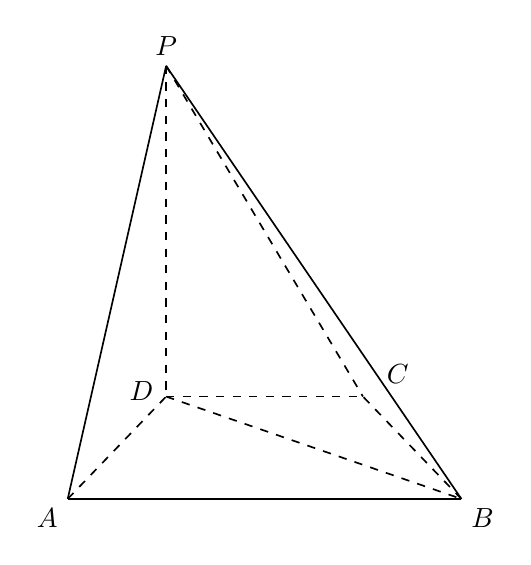
\begin{tikzpicture}[line width=0.6pt, font=\normalsize]
\coordinate (P) at (1.2500000000,6.0000000000);
\coordinate (D) at (1.2500000000,1.8000000000);
\coordinate (C) at (3.7500000000,1.8000000000);
\coordinate (A) at (0,0.5);
\coordinate (B) at (5.0,0.5);
% base trapezoid
\draw (A) -- (B);
\draw[dashed] (A) -- (D);
\draw[dashed] (D) -- (C);
\draw[dashed] (B)--(C);
\draw[dashed] (D) -- (B);
% lateral edges
\draw (P) -- (A);
\draw (P) -- (B);
\draw[dashed] (P) -- (D);
\draw[dashed] (P) -- (C);
\node[above] at (P) {$P$};
\node[left,xshift=-1.0pt,yshift=2pt] at (D) {$D$};
\node[right,xshift=5pt,yshift=8pt] at (C) {$C$};
\node[below left] at (A) {$A$};
\node[below right] at (B) {$B$};
\end{tikzpicture}
